\documentclass[review]{elsarticle}

\usepackage[utf8]{inputenc}

\usepackage{lineno,hyperref}
\modulolinenumbers[5]

%% Change to final when definitive version of the paper will be generated.
\usepackage[draft, lang=spanish, mode=multiuser]{fixme}

\FXRegisterAuthor{kcmd}{kenv}{klyone}
\FXRegisterAuthor{jcmd}{jenv}{jda}
\FXRegisterAuthor{fcmd}{fenv}{felipetg}

\journal{Journal of \LaTeX\ Templates}

%%%%%%%%%%%%%%%%%%%%%%%
%% Elsevier bibliography styles
%%%%%%%%%%%%%%%%%%%%%%%
%% To change the style, put a % in front of the second line of the current style and
%% remove the % from the second line of the style you would like to use.
%%%%%%%%%%%%%%%%%%%%%%%

%% Numbered
%\bibliographystyle{model1-num-names}

%% Numbered without titles
%\bibliographystyle{model1a-num-names}

%% Harvard
%\bibliographystyle{model2-names.bst}\biboptions{authoryear}

%% Vancouver numbered
%\usepackage{numcompress}\bibliographystyle{model3-num-names}

%% Vancouver name/year
%\usepackage{numcompress}\bibliographystyle{model4-names}\biboptions{authoryear}

%% APA style
%\bibliographystyle{model5-names}\biboptions{authoryear}

%% AMA style
%\usepackage{numcompress}\bibliographystyle{model6-num-names}

%% `Elsevier LaTeX' style
\bibliographystyle{elsarticle-num}
%%%%%%%%%%%%%%%%%%%%%%%

\begin{document}

\begin{frontmatter}

\title{A PPS distribution system for SKA}
%\title{Elsevier \LaTeX\ template\tnoteref{mytitlenote}}
%\tnotetext[mytitlenote]{Fully documented templates are available in the elsarticle package on %\href{http://www.ctan.org/tex-archive/macros/latex/contrib/elsarticle}{CTAN}.}

%% Group authors per affiliation:
%\author{Elsevier\fnref{myfootnote}}
%\address{Radarweg 29, Amsterdam}
%\fntext[myfootnote]{Since 1880.}

%% Group authors per affiliation:
\author{Miguel Jiménez-López, Felipe Torres-González, Javier Díaz}
\address{CITIC, ETSIIT, University of Granada}

%% or include affiliations in footnotes:
%\author[mymainaddress,mysecondaryaddress]{Elsevier Inc}
%\ead[url]{www.elsevier.com}

%\author[mysecondaryaddress]{Global Customer Service\corref{mycorrespondingauthor}}
%\cortext[mycorrespondingauthor]{Corresponding author}
%\ead{support@elsevier.com}

%\address[mymainaddress]{1600 John F Kennedy Boulevard, Philadelphia}
%\address[mysecondaryaddress]{360 Park Avenue South, New York}

%\listoffixmes

\begin{abstract} 
	The present paper describes the PPS distribution system for the Square Kilometer Array. The system architecture is described in depth. 
\end{abstract}

\begin{keyword}
	Square Kilometer Array, White Rabbit, Synchronization, Network
\end{keyword}

\end{frontmatter}

\linenumbers

\section{Introduction}

\jcmdnote{We have to add more information to this introduction...}

There are many mechanisms to distribute time information and signals. Some of them use GNNS receivers to get timing from the Satellites (GPS, Glonass, Galileo) meanwhile others use wired protocols to provide the time reference through the network. In all these cases is important to note that it is not the same to distribute frequency than distributing phase information. The first problem is about sending the oscillator signal through a wire or provide a mechanism to regenerate the clock frequency and usually is called synthonizaton. On the other hand, the latter ensures that in all the elements of a network the events trigger exactly at the same instant and is known as synchronization. In the phase distribution scenario, the phase information is encoded on a pulse that is transmitted thought the wire periodically each second and use this as reference to know when a new second starts. This is typically called PPS (Pulse Per Second) signal. Finally, the last problem is the provision of the time that is not only ticking at the same time, having the same reference about when to start the counting but also having the same time in all the devices. This can be distributed by propagation of the time information from a central time server and then, by measuring the propagation time of this message, annotating it in each node. A network is synchronized when takes into consideration these three elements: frequency, phase (PPS) and time.

This contribution is focused on finding a solution to provide ultra-accurate PPS signal distribution for the Square Kilometer Array (SKA) Telescope \cite{ska:project_website}. It is an international project to build a radio telescope tens of times more sensitive and hundreds of times faster at mapping the sky than today’s best radio astronomy facilities. It will become the world’s largest radio telescope. But the SKA is not a single telescope, but a collection of various types of antennas to be spread over long distances. Once completed, it will generate data at a rate more than 10 times today’s global Internet traffic. The SKA will be used to answer fundamental questions of science and about the laws of nature and imposes a technological challenge never faced before. 

This article presents a new device based on the technology called White-Rabbit \cite{ohwr:wr_wiki} to be used as mechanism for ultra-accurate PPS signal distribution. Section 2 will present the SKA Telescope project, the different network and the timing requirements that explain why an industrial technology solution is not feasible for SKA. Section 3 focuses on the fundamentals of the White-Rabbit technology. Section 4 describes the proposed node as end-node for SKA Telescope including the justification, architecture and software support. The synchronization performance under different scenarios, network topologies and environmental conditions are finally presented on section 5 illustrating the goodness of the exposed solution. Final remarks are described on the section 6. The last sections are dedicated to the conclusion, future work and the acknowledgments.

\jcmdnote{Add some reference about the commercial synchronization solutions.}

\section{The SKA telescope}

The Square Kilometer Array (SKA) will be the largest radio-telescope of the world. Located in two different geographical areas (South-Africa and Australia/New Zeland) it will be one of the great physics machines of 21st Century and, when complete, one of the world’s engineering marvels. It will be constructed on different phases SKA1 (phase 1 2018-2023) and SKA2 (phase 2 2023-2033). The development will be deployed using on two different pathfinders existing on each place (MeerKAT in South Africa and ASKAP in Australia). 

The key science goals for this instrument are:

\begin{itemize}
	\item {Formation of the 1st galaxies in a dark Universe dominated by atomic gas.}
	\item {Evolution of the atomic gas till the current epoch.}
	\item {Strong Field Tests of Gravity Using Pulsars and Black Holes.}
	\item {Acceleration in the expansion of the Universe not understood yet.}
	\item {Habitable extra-solar planets (proto-planetary disks, biomarkers).}
\end{itemize}

The SKA facility will use several kind of antennas targeting different geographical locations and time schedule. During SKA1 and according to the SKA1 System Baseline description \cite{ska:baseline_description_v2}, for building such facility two different kinds of antennas will be used according to their capabilities to sense. They are: 

\begin{itemize}
	\item {SKA-LOW, 50 - 350 MHz Australia, 131,000 aperture array dipole 512 stations of 256 antennas.}
	\item {DISHES, 350 MHz - 14GHz South-Africa SKA1\_Mid 350 MHz – 14 GHz 64 MeerKAT dishes plus additional 133 SKA1 dishes.}
\end{itemize}

\begin{figure}[h]
	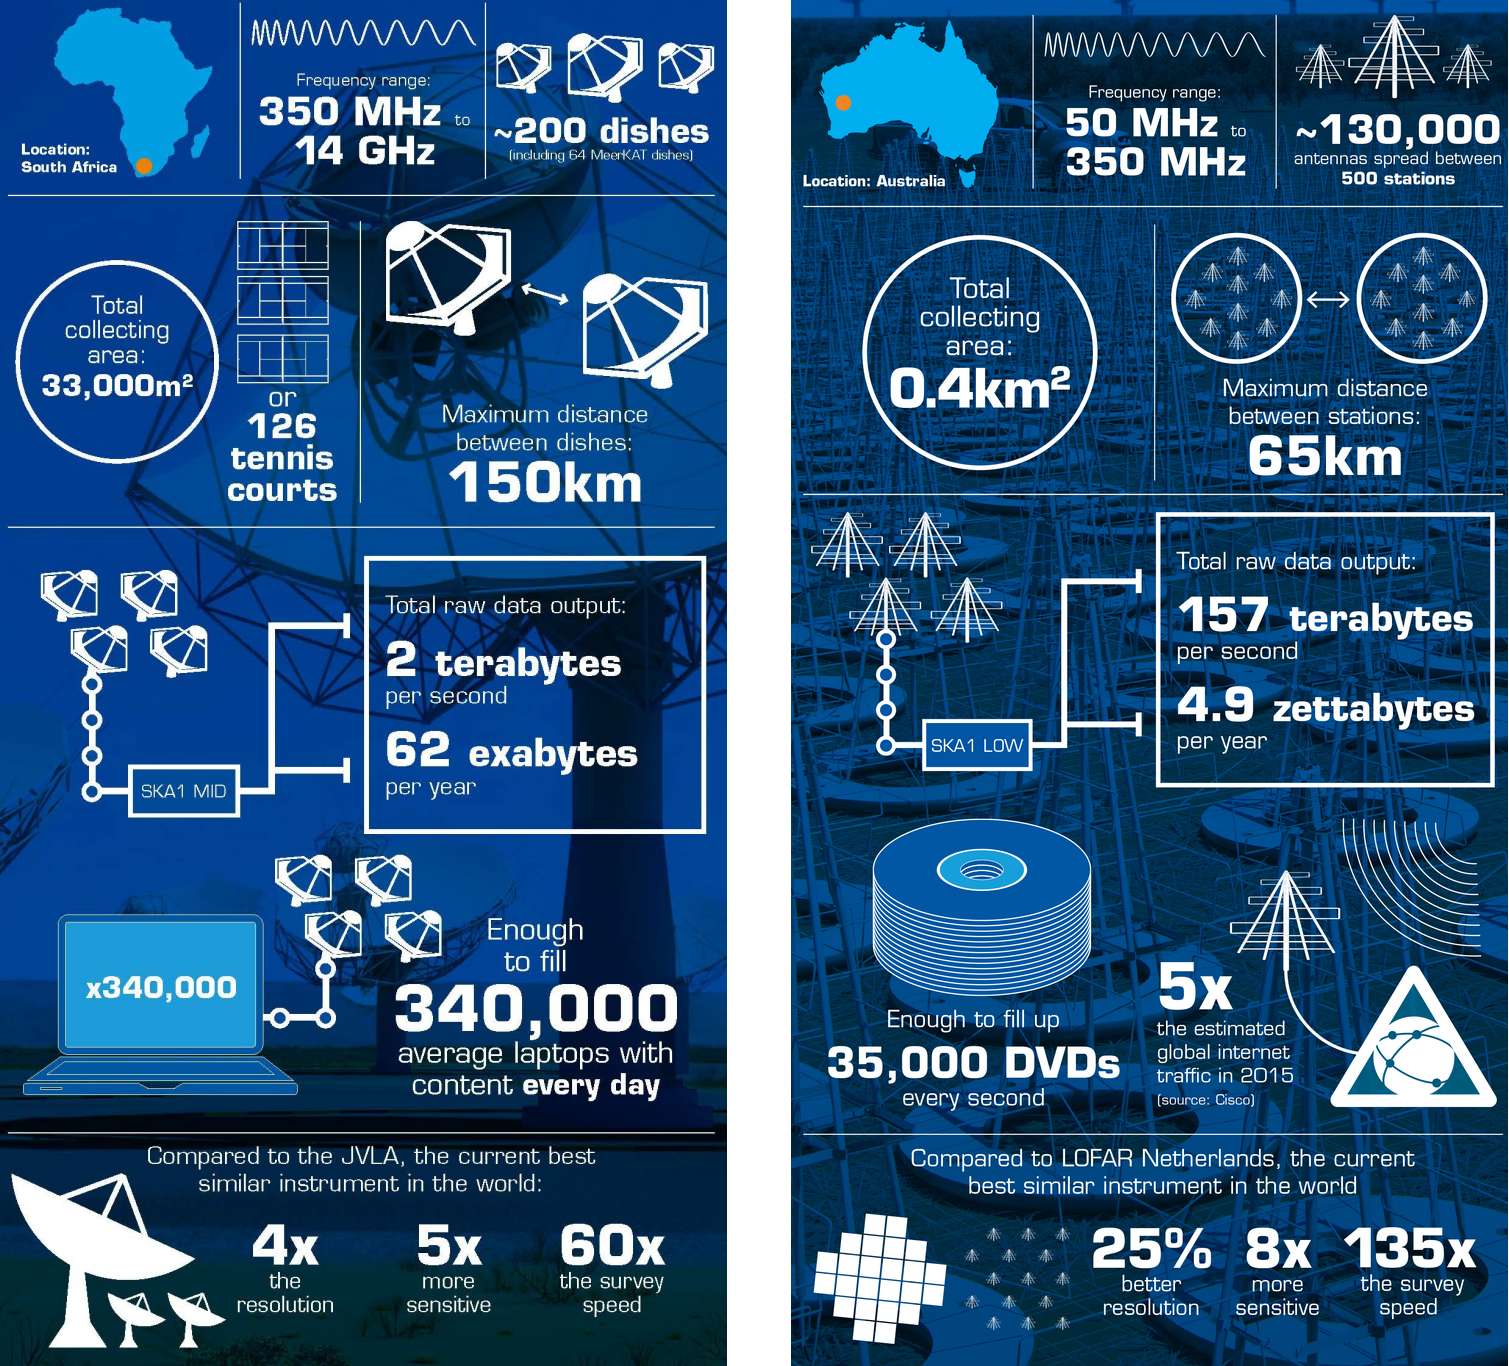
\includegraphics[scale=0.25]{img/ska_instruments}
	\caption{The SKA's low frequency (right) and the mid-frequency (left) instruments.  SKA Telescope will be built on two different phases. These images (adapted from \cite{ska:multimedia_rsrcs}) illustrate key numbers corresponding to SKA1 phase (starting 2018). }
	\label{fig:ska_instruments1}
\end{figure}

The SKA1 telescope is being designed to optimize its performance and some key facts about both types of instruments are shown on Fig. \ref{fig:ska_instruments1}. 

The scale of the SKA Telescope represents a huge leap forward in both engineering, research and development towards building and delivering a unique instrument, with the detailed design and preparation now well under way. The unprecedented high performance specifications requires the utilization of best technologies and design strategies possible and represent an unprecedented challenge for all the elements to be built. 

\subsection{SKA Telescope Network}

The SKA Telescope use different types of networks to guarantee a proper operation of the infrastructure. The design of the network corresponds to the Signal and Data Transport (SaDT) element \cite{ska:sadt_website} and it includes all hardware and software necessary for the transmission of data and information between the Elements of the SKA. SADT also contains details about the provision of timing which is critical for interferometry.
The data network includes the Digital Data Backhaul (DDBH) that transports signals from the radio telescopes to the Central Signal Processor (CSP), and data products from the CSP to the Science Data Processor (SDP) and from the SDP to the regional SKA Data Centers. The total data rates are very high, approximately 80 Tb/s for the DDBH links and another 80Tb/s for the CSP links. 
Also covered by the SaDT is the Monitor and Control (M\&C) that transmits and receives monitoring and control information throughout the system and includes the Telescope Manager, itself comprised of three logical networks: Production Network, Engineering Network and Safety Network, the Network Manager as well as local monitoring and control.

The final part of the SaDT is the Synchronization and Timing (SAT) that provides frequency and clock signals from a central clock ensemble to all elements of the system to maintain phase information to the required accuracy for all receptors, and timing signals for data identification and time critical activities at the receptors, and the CSP and SDP. To maintain phase coherence across the array requires short-term timing precisions of around 1 ps, while for the requirements for the long-term timing for pulsar require 10 ns accuracies over 10 year periods. The timing is critical to the functionality of the SKA to work as a unified large telescope using a technique known as interferometry. This contribution will focus on the high accuracy synchronization method used for SKA1 responsible to provide a PPS (Pulse Per Second) signal to the critical elements. 

\begin{figure}[h]
	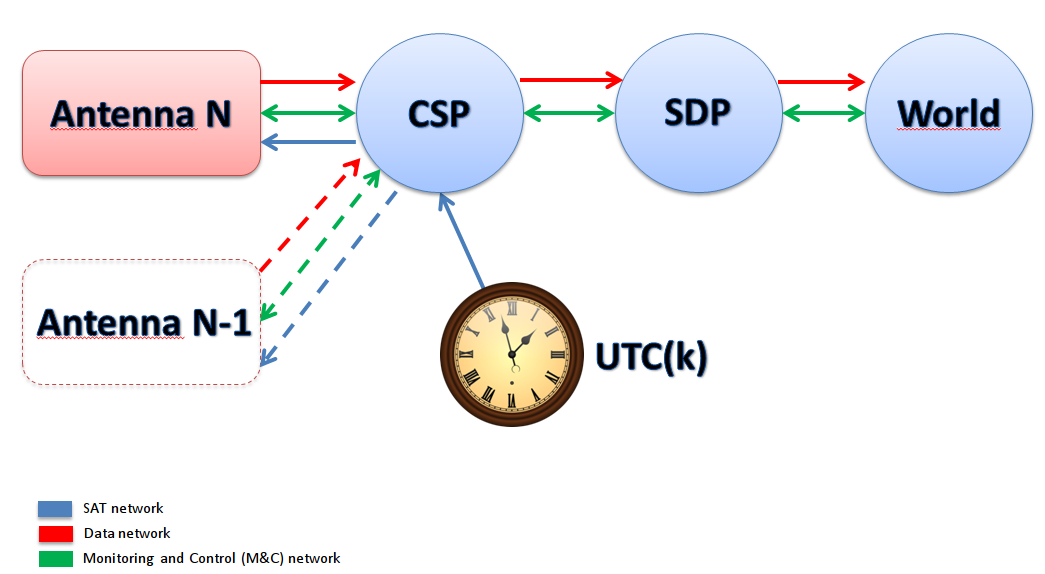
\includegraphics[scale=0.4]{img/ska_network_arch}
	\caption{The SKA Telescope network architecture is composed by three networks: the data network (red), the M\&C network (green) and the SAT network (blue). An external clock reference, UTC traceable, is provided to the whole Telescope elements in order of providing an unique time reference.}
	\label{fig:ska_net_arch1}
\end{figure}

\jcmdnote{This figure must be re-made because it is not ours. It would be convenient to use the same terminology than figure's caption...}

\subsection{Distribution of high accuracy timing signals for ska1}

As determined by SaDT, SKA telescope should be able to distribute a commune frequency reference to all the telescopes and, in addition, provide a uniform time reference to register all the events with ultra-high accuracy through time stamps. This task is done by the SAT (Synchronization and Timing) element that belongs to SaDT. The SKA timescale is maintained by the central clock ensemble for each telescope and will be steered to within designed limits of UTC (Coordinated Universal Time) and monitored with respect to UTC via GNSS time transfer techniques. These clock ensembles form the fundamental timescale for SKA and will be the basis for precision measurements of pulsars and other time-dependent phenomena. As consequence, during this distribution, UTC refers to UTC (SKA), as realized by the central SKA clock ensemble.
This article will focus on the solutions to distribute the UTC time by means of PPS (Pulse-Per-Second signal). This PPS signal guarantees that all the scientific data are time-tag using a common reference. This time reference has high requirements coming from science that are not mandatory by other elements of the SKA systems as the monitor and control network. For these other elements, standard time transfer protocols as NTP or IEEE-1588 are a feasible solution. For the Telescope core, we illustrate that the high performance requirements imposed by the challenging scientific goals force to provide much more sophisticated solutions. 
The PPS distribution system will be in charge to deliver its output at the following locations:

\begin{itemize}
	\item {Each of the 133 dishes of SKA1-MID, and once to the Meerkat system. The maximum receptor baseline lengths are between 120-150 km.}
	\item {The core of SKA1-LOW, and the 45 stations in total along the 3 spiral arms. The maximum receptor baseline lengths are between 70-80 km. }
	\item {The encoded absolute time signal will be delivered to each of the three CSPs.}
\end{itemize}
 
Note that if the offset frequency scheme is to be applied to all SKA1-Mid dishes, an additional 64 STFR endpoints will be needed in SKA1-mid. This provides between 182 and 246 endpoints to synchronize. 
The general array SAT requirements for the frequency distribution is 1 ps while the time synchronization and time-stamp requirement is 10ns. SaDT uses different mechanisms for achieving goals, frequency dissemination and PPS distribution. As consequence, because the goal in this contribution is just describing a solution for PPS distribution, the contribution work only considers the second requirement, the 10 ns synchronization as needed for example for the long-term timing Pulsar studies. Note that a complete description of the SKA network elements and topology is out of the scope of this contribution and only the requirements needed is presented to properly understand the need of the solution here developed. 
It is important to remark than the 10 ns requirement is the time-budget allocated for the whole network. Because elements such as main clock also consume part of this budget, it translates into PPS-distribution time requirement of 5 ns. The error here includes PPS distribution, delay center precision, Dish timing transport and time-stamping errors. This time-budget should be distributed on the different elements of the system that rely on the network topology that determine the number of hops. Based on current SAT network topology, the target specification for the elements of the PPS distribution system provides them an average time-budget better than 2 ns. This is a quite challenging goal not only because impose a high accuracy synchronization goal but especially having into account the installation environmental conditions. The SKA1 use aerial optical fiber networks that are significantly affected by the large temperature excursion during operation, more than 50º due to the installation on desert locations of Sud-Africa and Australia. Furthermore the outdoor wind velocities during normal operation could achieve up to 40 km/h. it makes the fibers oscillate, changing their length, which must be compensated on real-time during execution or averaged them out. 
Next section will provide the description of the solution proposed to be use on SKA1 as mechanism for PPS distribution. 

\section{The White Rabbit synchronization protocol}

The White Rabbit (WR) protocol is an open hardware/software technology that improves the Gigabit Ethernet (GbE) and Precise Time Protocol version 2 (PTPv2) for optical fiber links. Its main goal is to provide a timing synchronization with an accuracy better than a nanosecond and the precision in the scale of picoseconds. WR implements mechanisms to ensure the deterministic and reliable data transfer between thousand of nodes connected with large links up to 10 km. As conventional networks, WR proposes a hierarchical topology with a root node that is responsible for distributing the reference clock to other devices. This element is known as Grand Master and it is driven by a GPS or atomic clock. The intermediate levels of the network are composed of WR Switches that are multi-port devices and behave as PTPv2 Boundary Clock (BC). The different ports of the WR Switch are divided on two types: one of them is the slave (uplink) and connects the Switch with the upper layer and the other ports are masters (downlinks) and they are charged to propagate the synchronization to the next level of the hierarchy. The nodes of the last level of the network are known as Slave devices and its main purpose is recovering the clock signal of the link and synchronizes its local oscillator.

\kcmdnote{Add figure to show the WR topology.}

WR is based on other technologies such as Synchronous Ethernet (SyncE), an extension of PTPv2 (WR-PTP) and additional phase alignment techniques. The SyncE allows the physical layer of the Ethernet to transmit the master clock inside the data stream. Then, the slave nodes can recover it and configure their local oscillators to follow it. The WR-PTP implements extra messages in the PTPv2 and it is proposed to be included in the new PTP release (PTPv3) as a High Accuracy profile. WR also uses additional phase alignment techniques as the Digital Dual Mixed Time Difference (DDMTD) that is a module responsible for measuring the phase between two clocks. This information is used to change the frequency of the local oscillator for the synchronization process.

WR is designed to be use in a Field Programmable Gate Array (FPGA) device and the source code is mainly written in HDL languages such as VHDL or Verilog. Moreover, there are several platforms that can implement WR that ensures the vendor-independent feature of WR. The main Intellectual Property (IP) block is the WR PTP core (WRPC) for WR nodes and the Real Time Subsystem (RTS) for WR switches. The most common WR nodes are based on carrier boards such as SPEC or SVEC and can be plugged in a PCIe/VME socket of a conventional PC. Some WR nodes have a standalone mode but in this case they can not benefit of high level features usually provided by a PC CPU.

\kcmdnote{Here, I am not sure if we have to describe a little the WR-ZEN because in next section will be discussed in detail. However, we have to present it and I think that maybe some information can be repeated.}

The WR Zynq Embedded Node (WR-ZEN) is a new generation board that brings a Xilinx Zynq System-on-Chip (SoC). The Zynq SoC is composed of a FPGA and a hard ARM dual core microprocessor that can run a \textsc{bare-metal} application or a standard Operating System such as Linux. The WR-ZEN has been proposed to be used in the SKA project to implement the PPS distribution system that will be discussed in detail in the next section.

\section{The PPS distribution system for SKA}

%% ---------------- From WR-ZEN article (EFTF2016) ------------------------
%
%The WR-ZEN is a new kind of WR node that incorporates
%a FPGA device and a hard ARM dual core microprocessor
%inside the same chip. The ARM is able to run a Linux kernel
%and this eliminates the need to use a conventional PC with an
%operating system. The flexibility of the platform has motivated
%that WR-ZEN is under study to be used in important scientific
%infrastructures such as Square Kilometer Array [11] (SKA)
%and Cherenkov Telescope Array [12] (CTA) among others.
%
%% ------------------------------------------------------------------------

The PPS distribution system for SKA is based on the WR-ZEN platform that provides the WR support in order to ensure the synchronization accuracy in the system. The first design of the PPS system includes the Fine Delay FMC card that is used to generate the timing signals to be transmitted over the link. Moreover, Network Interface Card (NIC) capabilities have been added to the design and their two optical fiber ports can be accessed as conventional Linux network interfaces.

\subsection{Hardware}

%% ---------------- From WR-ZEN article (EFTF2016) ------------------------
%
%The WR-ZEN is a small stand-alone board that integrates
%the latest Xilinx Zynq Z-7015 device with a Dual ARM
%Cortex-A9 MPCore with CoreSight and containing an Artix
%FPGA-logic with 74K logic cells, 380KB of embedded mem-
%ory and 160 DSP blocks. It has two optical SFP Ethernet
%interfaces, two copper Ethernet ports and the FMC expansion
%connector. On addition to FMC, a SAMTEC connector is
%available for developing of simple expansion boards and some
%USB sockets for monitoring. The WR-ZEN node is provided
%with improved oscillators, PLLs and a clocking scheme that
%provides significant better short term stability than previous
%WR node designs. It also includes several SMA outputs that
%can be configured to generate signals from the FPGA and an
%input that allows the WR-ZEN to behave as grandmaster. The
%WR-ZEN can be used with several FMC cards depending on
%the application: ADC, DAC, TDC, DDS, Fine delay, Digital
%I/O, etc.
%
%% ------------------------------------------------------------------------

The WR-ZEN is a board designed by Seven Solutions company and contains a Xilinx Zynq SoC. This SoC has a ARM dual core microprocessor (Cortex-A9 MPCore with CoreSight) and a FPGA device (Artix with 74K logic cells, 380KB of embedded memory and 160 DSP blocks). This versatile architecture removes the necessity of a conventional PC because all the high-level software components can be implemented in the on-board processor. The WR-ZEN has been conceived with an improved clocking scheme in relation to older WR nodes. \kcmdnote{Felipe, here you can explain in depth the clocking circuitry and show the improvements in relation to older WR nodes such as SPEC.} It takes into advantage of better oscillators and additional PLL to be capable to generate a wide range of frequencies for several kind of different applications. The WR-ZEN is fully connected thanks to its two optical fiber SFP interfaces and two RJ45 sockets and has other standard ports such as FMC, SAMTEC, UART, I2C, SPI, etc. The expansion connectors (FMC and SAMTEC) are though to add other boards that implement specific features or capabilities. Typical applications for the FMC mezzanine board are Analog to Digital Converter (ADC), Digital to Analog Converter (DAC), Time to Digital Converter (TDC), Fine Delay, Digital I/O (DIO), etc. The SAMTEC connector is used to add extra circuitry to provide redundancy (duplicate power supply) and other additional components such as fans, LCD display, power supply control chips, etc.

\kcmdnote{Add WR-ZEN photo.} 

\subsection{Gateware}

%% ---------------- From WR-ZEN article (EFTF2016) ------------------------
%
%The gateware refers to the design that must be programmed
%in the Programmable Logic (PL) and the Processing system
%(PS) configuration to be applied. The PL is based on the Wish-
%bone (WB) bus [13] and has a main crossbar that interconnects
%the different IP cores.
%In the Fig. 2, the PL architecture is represented in more
%detail.
%* GIGABIT TRANSCEIVER PORTS (GTP): These
%blocks contain primitives to transfer data through a
%high performance dedicated interfaces. The GTPs are
%connected to the SFP sockets and allow to send/receive
%packets to/from the Gigabit Ethernet network.
%* WR PTP DUAL PORT CORE (WRPC-2P): It is the
%key core for WR nodes and contains all the elements
%needed to implement the WR protocol for two optical
%fiber ports.
%* AXI TO WB BRIDGE (AXI-WB BRIDGE): The PS
%must be able to talk to the PL. However, the PS
%uses the AMBA/AXI bus specification instead of the
%WB one of the PL. The AXI-WB bridge is able to
%convert from WB transactions to AXI transactions and
%viceversa.
%* FMC CORE: This IP core gives the specific function-
%alities for a certain kind of FMC card. In the reference
%design, the Fine Delay FMC core is included.
%* NETWORK INTERFACE CORE (NIC): It provides a
%network controller that is directly accesible from the
%Linux kernel. The NIC module can be managed like a
%standard network interface thanks to a specific driver.
%The gateware design carries out a WR compliant node
%with network capabilities and support for several FMC cards.
%However, the reference design only uses the Fine Delay FMC
%card, it can be extended easily to work with other cards such
%as DIO, TDC, ADC, etc.
%
%% ------------------------------------------------------------------------

The term gateware is referred to the reference architecture with all the components that will be synthesized in the FPGA device. It is built on two different levels. The former uses the AMBA bus specification and considers the main elements for the Zynq ecosystem with several components such as Zynq Processing subsystem that takes care of configuring the ARM microprocessor and controlling the bus interconnections with it, a reset and clocking module that manages the clock and reset signals, an AXI QSPI core to program the hardware PLL chip, an AXI crossbar to glue everything together and a specific IP core that represents the next level of the design that is explained in following lines.

\kcmdnote{Add figure to show first level architecture.}

The second level is referred to the specific IP core that takes into consideration the WR protocol and other basic features such as Gigabit networking, serial debug communication, Timestamp mechanism, etc. This module uses the Wishbone Open Cores bus specification and is mainly vendor-independent. It is composed of many IP cores that are interconnected through a WB crossbar that allows bidirectional communication between any two IP cores. Moreover, the crossbar can store Self Descriptor Bus (SDB) information about the different components attached to it in order to discover them with a scan operation. Thanks to it, the WB peripherals can be discovered automatically by software tools and this allows not to hard-code the different addresses inside the source code improving the maintainability of the system. The main modules at this level are the following:

\kcmdnote{Add figure to show second level architecture.}

\begin{itemize}
	\item{\textbf{AXI-WB bridge:} It converts transactions between WB and AXI buses. This is important because the Zynq Processing System is thought to use the AXI bus and the original project of WR was developed with the Open Core WB bus. }
	\item{\textbf{\kcmdnote{Add figure to show WRPC-2P architecture}WR Dual Port core:} It is most important module for WR nodes and it is charged to implement WR functionalities. Its internal architecture includes a soft-microprocessor (LM32) that runs a specific bare-metal firmware with WR functions/capabilities stored in the WB RAM core. The WR endpoints include some state machines to manage Ethernet packets of a Gigabit network. The Mini-NIC core receives and sends WR-PTP packets from/to network. The WB Syscon is the general controller of the system that manages communications protocols such as UART, I2C or 1-Wire and contains system control registers too. The WB PPSgen contains the timebase counter for the WR technology and the SoftPLL that is a special component that perform phase measurement between different clocks and has a PI control loop to set up the DAC chip on the board to change the local oscillator frequency. }
	\item{\textbf{WB Crossbar:} It is responsible to connect all the modules together in order to allow communication between them. However, the real design is more complex because it has several WB crossbar at different hierarchy levels. }
	\item{\textbf{GT modules:} Gitabit Transceivers are device specific primitives to implement the high speed interfaces. They are used to create two Gigabit Ethernet ports for optical links through SFP modules.}
	\item{\textbf{NIC components:} They are responsible to receive/transmit Ethernet packets from/to the network. Nevertheless, its initial design is not suitable for high bandwidth interfaces because it does not incorporate a DMA controller. 
	%This feature is planned future improvement for the project.
	}
	\item{\textbf{TxTSU core:} When a packet is received from the network, the timestamp is appended to it as Out-of-Band (OOB) data. So, the software driver in the ARM can recover this information reading it from the packet. However, for the transmitted packets, this mechanism is not possible. To solve this problem, a Transmit Timestamp Unit is added to the design. Its main purpose is to store timestamps for outgoing packets in a FIFO memory until the ARM accesses them. Thanks to this trick, we can get the timestamp for every packet. 
		
	%At this point, there are other enhancement to be into consideration. The timestamp granularity is limited by the clock %frequency of the system. An interesting task is to extend the precision to nanosecond scale as White Rabbit technology %promises.
	}
	\item{\textbf{Fine Delay FMC module:} It is a controller for the Fine Delay FMC mezzanine card. The main task of this board is to configure a delay to transmit a signal from the TTL trigger buffer to one of its four outputs. The delay range is between 600 ns and 120 s with a resolution of 1 ns. In addition, more complex mode can be programed and a wide variety of signal can be generated.}
	\item{\textbf{WB I2C arbiter:} This simple module multiplexes several I2C bus transactions that have to use the same I2C physical bus. It is necessary because the WR-ZEN only have an I2C bus accessible from the FPGA device.}
\end{itemize}

\subsection{Firmware}

The LM32 soft-microprocessor is responsible for implementing the WR protocol. The code is written in C language and considers low level hardware drivers for each IP core and the WR-PTO that includes the PTPv2 stack with some add-ons for WR. In addition, a simple Command Language Interface (CLI) is introduced to allow the user interaction (think that some WR nodes can work in standalone mode and does not have an on-board hard microprocessor). The main tasks for the WR firmware is to implement the WR-PTP protocol and the control routines of DAC chips. 

\kcmdnote{What more information can we add at this point?}
%% More information about WR-PTP??
The WR-PTP is implemented in two flavours: PTP-no-POSIX and PTP Port to Silicon (PPSo). The former is a simple version as its name indicates, is not POSIX compliant. This is the old implementation and it has been replace with the PPSi that is POSIX compliant.

The PI loop for DACs is coded using an LM32 IRQ handler for the SoftPLL module. The SoftPLL measures phase differences between clocks as we discussed in the previous section. Taking into account this information, a PI loop algorithm is performed to calculate the value to be applied to each DAC chip in order to change the local oscillator frequency to follow the master one (in a slave mode). One thing to be into consideration is that the process must be determinism and it only can be ensured if there is only an interrupt source and nothing can stop the SoftPLL operation.

\subsection{Software}

%% ---------------- From WR-ZEN article (EFTF2016) ------------------------
%
%In this section, the software components needed to run a
%Linux kernel/Baremetal application on the WR-ZEN board are
%described. The Zynq devices needs a binary file (BOOT.bin)
%that is composed of a specific Xilinx bootloader known as First
%Stage Bootloader (FSBL), a gateware bitstream to program
%the FPGA and a baremetal application or a Second Stage
%Bootloader (SSBL) if Linux kernel must be loaded. The FSBL
%is encharged to initialize different peripherals, configure the
%FPGA with a bitstream and run the baremetal application
%or the SSBL. The baremetal application is encouraged to be
%coded with the Xilinx SDK because all the gateware details
%are imported to the software project and we can use all the
%functionalities of the Xilinx Board Package Support (BSP). On
%the other hand, the SSBL is a independent project and must be
%downloaded and compiled separately. The most common SSBL
%are U-boot [14] and Barebox [15]. The chosen bootloader is U-
%boot instead of Barebox because there is a Xilinx repository
%[16] that includes custom code for the Zynq devices. When
%everything is generated, the Xilinx SDK or bootgen tool must
%be used to pack all the binaries in a single file, the BOOT.bin.
%The following step is to compile the Linux kernel, kernel
%modules, libraries and userspace tools. To face this task, there
%are two ways. The first one is to compile every component
%separately and manually. It is very slow, tedious and error
%prone but it is the best way to control the different steps
%and customize them if necessary. On the other hand, there
%are some tools that automate the process such as Yocto [17]
%or Buildroot [18]. However, they present a disadvantage: the
%user loses the control and it is more difficult to add some mod-
%ifications because the tool does everything automatically. For
%the reference design, the Buildroot is used to ease and speed
%up the compilation of the Linux kernel, U-boot bootloader, the
%kernel modules and userspace tools. The Buildroot package is
%retrived from the official project website. It is very configurable
%and includes the Kconfig support to enable/disable the different
%features similar to the Linux kernel. Although the Buildroot
%eases very much the compilation process, it has many options
%and may be confusing for a non-expert user. To solve this
%issue, a set of scripts have been implemented to perform all
%the actions needed and configuration files for the Busybox,
%Linux kernel and the Buildroot are provided. This scripts are
%based on others from the WR Switch Software project [19] of
%the OHWR repository.
%In addition of the Linux kernel and the bootloader, some
%kernel modules and userspace tools for the WR-ZEN board
%have been written. The main kernel driver is the WR-ZEN
%carrier, known as zen, and is responsible for reprogramming
%the FPGA device and reading the EEPROM information of
%the WR-ZEN board. This driver is based on the fmc-bus
%[20] (OHWR) and it also gives NIC capabilities to manage
%the optical fiber ports as standard network interfaces from
%the Linux kernel. Some userspace tools to read/write the
%FPGA register (zenmem), reprogram the FPGA bitstrean (zen-
%fwloader.sh), reprogram the soft-microprocessor program (zen-
%cl) and send commands to the soft-microprocessor (zen-vuart)
%are included too. The driver and all these tools are inspired by
%the SPEC Software project [21] of the OHWR repository. As
%we saw in the previous section, the reference design has also
%a Fine Delay core that must be controlled by a specific kernel
%driver. Actually, there are two drivers (zio [22] and fmc-fine-
%delay [23]) and some userspace tools in the OHWR for the
%Fine Delay FMC card in a SPEC card. Using these ones as
%starting point, some minor modifications have been made to
%incorporated them to the WR-ZEN reference design.
%
%% ------------------------------------------------------------------------

The WR-ZEN can take advantage of having a hard dual core microprocessor because it allows to deploy a Linux system in the platform or a baremetal application that manages the hardware resources directly. In the SKA system, the WR-ZEN is used with a Linux kernel to implement the specific applications needed by the system. To accomplish this task, a process must be defined to build the kernel and all software components (daemons, applications, drivers, etc) in a simple and automatic way. The manual building of the Linux system is not an acceptable procedure because it requires human-intervention and it is complex, tedious and error prone task. Other solution could be to use an existing software tool (Buildroot or Yocto for example), however, it used to have some customization limitations. On the other hand, a custom and automatic building system could be coded but it often carries creating several scripts and this task is high time consuming. The final solution is a mixed scheme: a software tool known as Buildroot and some scripts to perform additional tasks. Buildroot is responsible for generating a new Operating System based on Linux with multiple applications and the root file system to get a fully operational environment. However, its main disadvantage is the lost of control due the fact all the steps are automatic and it has advanced topics that are difficult for newbies. To solve these inconveniences, some custom scripts (inspired by WR Switch Software project ones from OHWR) are added to allow user intervention and provides standard configuration for Linux kernel, Busybox and root filesystem. The Busybox is a software package that contains most used and important tools in Linux environment. Nevertheless, it is optimized for embedded devices because it only generates a single binary for all tools. The root filesystem is the main file holder for Linux system and it stores many files including tools, drivers, configuration files, initialization scripts, etc. Moreover the basic Linux components, some userspace tools and custom kernel drivers have been developed to manage the main modules in the WR-ZEN reference design. The kernel drivers that have been used, modified or implemented from others are the following:

\kcmdnote{Add figure to show device driver relations.}

\begin{itemize}
	\item {\textbf{fmc:} It is retrieved from OHWR repository and it has not been modified. Its main purpose is implementing a generic support for FMC bus in the Linux kernel. It is necessary because many other drivers such as Fine Delay FMC one use its generic functions.}
	\item {\textbf{zen:} It is the main driver for the WR-ZEN board. It manages all the IP cores in the design and provides advanced features such as character device methods, NIC capabilities integrated with the Linux networking subsystem, reprogram the FPGA with the reference design, etc.}
	\item{\textbf{zio:} It is retrieved from OHWR repository and it has not been modified. It creates the ZIO bus that exports its attributes through the SysFS. The Fine Delay FMC driver is located at the top of the \textit{zio} one.}
	\item{\textbf{fmc-fine-del:} It is based on the OHWR repository version and includes some modifications to work properly in the WR-ZEN platform. It controls the Fine Delay FMC core and allows to set up the different working modes. An important consideration about this driver is the reprogramming of the FPGA with the Fine Delay FMC bitstream through the \textit{zen} API.}
	\item {\textbf{zen-nic:} It is additional module that is charged to enable/disable NIC methods. However, it does not implement these functions because they are in \textit{zen} kernel module. The \textit{zen-nic} is necessary because the Fine Delay FMC driver reprograms the FPGA and for this reason, the network initialization can not be performed in the \textit{zen} module directly.}
\end{itemize}

As previously seen, there are dependencies between the different kernel drivers and it establishes the installation order. The \textit{zen} one depends on \textit{fmc}. The \textit{fmc-fine-del} needs \textit{zen}, \textit{zio} and \textit{fmc}. The \textit{zen-nic} only uses the \textit{zen}.


In addition to device drivers, there are several custom userspace tools related with drivers previous explained. Those that use the \textit{zen} driver API are \textit{zenmem} that is responsible for accessing memory map of the WR-ZEN IP cores, \textit{zen-fwloader} that programs the FPGA with a given bitstream, \textit{zen-vuart} and \textit{zen-cl} that allows talking to the soft-microprocessor (see the gateware section) and loading other firmware respectively. On the other hand, the  \textit{fmc-fine-del} driver has associated tools such as \textit{fmc-fdelay-board-time} that is used to get the current time, \textit{fmc-fdelay-pulse} that generates pulses with certain characteristics (frequency, initial delay, duty cycle, etc), \textit{fmc-fdelay-input} that prints some information when an incoming signal raises the input connector of the mezzanine card, \textit{fmc-fdelay-list} that enumerates the Fine Delay FMC cards plugged in the system (only one for WR-ZEN but however more for conventional PCs), \textit{fmc-fdelay-status} that check the status of Fine Delay FMC core and \textit{fmc-fdelay-term} that configures the termination of each channel among others.

Apart from the Linux or baremetal environment described before, more components are needed  for the WR-ZEN platform. Previously any application or Operating system can run, a specific bootloader must initialize some hardware devices. In the Zynq technology, there is a special bootloader known as First Stage Bootloader (FSBL) that is responsible for early initializations and it is the first step to perform in whatever system based on Zynq. The FSBL sets up different peripherals, configures the FPGA with a bitstream and runs the baremetal application or the Second Stage Bootloader (SSBL). The most common SSBL are U-boot and Barebox. The chosen bootloader is U-boot instead of Barebox because Xilinx company provides custom code for the Zynq devices. Finally, the FSBL, bitstream and SSBL/baremetal application must be packed in a binary file named BOOT.bin using the Xilinx SDK environment or bootgen tool and put it in a FAT-32 (boot and lba flags enabled) partition of a SD card.

\kcmdnote{Add figure to show a software overview.}

\section{Test}

\section{Results}

\section{Conclusion}

\section{Future work}

\section{Acknowledgments}

\kcmdnote{Cite Manolo's projects if you do not want to die... Forever...}
The authors would like to thank to the CERN BE-CO-HT group, the WR community, the Seven Solutions staff and
other institutions such as JIVE (especially Paul Boven) for its collaboration testing the
WR-ZEN board. This work has been partially funded by the Horizon 2020 (H2020) ASTERICS (grant number 653477),
VITVIR (TIC-8120, Junta de Andalucia) and AYA2015-65973-C3-2-R: "AMIGA6: gas in and around galaxies. Preparation for SKA science and contribution to the design of the SKA data flow. Signal and Data Transport (SaDT)" projects.

\section*{References}

\bibliography{mybibfile}

\end{document}